\chapter{Revisão Sistemática}\label{cap_trabalho_academico}
O termo Revisão Sistemática (RS) é utilizado para se referir a uma metodologia específica de pesquisa, desenvolvida a fim de identificar, avaliar e interpretar as evidências disponíveis relevantes para um determinado tema, ou questão de pesquisa, ou área de tópico, ou fenômeno de interesse \cite{biolchini2005, kitchenham2004}. A perspectiva conceitual mais ampla propõe uma abordagem definida em três fases principais, sendo estas, o planejamento da revisão, a condução da revisão e a apresentação dos resultados da revisão \cite{biolchini2005}. 

O planejamento da revisão define a identificação do que é necessário para a revisão e o desenvolvimento do protocolo que a direciona. A condução da revisão identifica a pesquisa, a seleção dos estudos primários, a avaliação da qualidade dos estudos, a extração e a síntese dos dados. E por fim a apresentação da revisão é a documentação de todo o trabalho executado \cite{kitchenham2004}.

Neste capítulo estão descritos os métodos e os resultados extraídos da revisão sistemática sobre sistemas de apoio à decisão para nutrição hospitalar, suas principais formas de gerenciamento e análise de dados e \textit{Key Performance Indicators} (KPI) utilizadas.

\section{Planejamento da Revisão}

Na fase de planejamento, baseando-se em \citeonline{biolchini2005}, foi construída a formularização das perguntas da pesquisa onde foram definidos o objetivo: analisar dados estratégicos sobre nutrição clínica em hospitais e as características de qualidade e amplitude da pergunta, as quais são apresentadas no \autoref{quadro_formularizacaoPergunta}.
\newline
\newline
\newline

\begin{quadro}[htb]
\caption{\label{quadro_formularizacaoPergunta}Formularização das questões.}
\label{}
\begin{tabular}{|p{3cm}|p{8cm}|}
	\hline
	\textbf{Problema}       & Entender a disponibilização de dados sobre o ambiente nutricional clínico-hospitalar no Brasil e no mundo e a qualidade dos dados disponibilizados para tomadas de decisões eficientes.  \\ \hline
	\textbf{Palavras-chave} & Gerenciamento, Análise, Dados, Acompanhamento, Nutricional, Hospital, KPI, Tomada de decisão, Apoio a decisão.   \\ \hline
	\textbf{Intervenção}    & Utilização de análise de dados e plataformas de \textit{Business Intelligence} em Hospitais e seus departamentos de Nutrição Clínica.   \\ \hline
	\textbf{Controle}       & Planilhas de 2019 das triagens realizadas pela unidade de nutrição clínica do HU/UFS.
 \\ \hline
	\textbf{Efeito}         & Referências de KPI utilizadas em estudos anteriores e/ou projetos de \textit{Business Intelligence} focados na área da nutrição. \\ \hline
	\textbf{População}      & Redes hospitalares. \\ \hline
	\textbf{Aplicação}      & Gestores de hospitais e departamentos de nutrição, nutrólogos, analistas de B.I.\\ \hline
\end{tabular}
\legend{Fonte: Autor.}
%\fonte{Autor.}
\end{quadro}

Com os requisitos de formularização da pesquisa definidos foram criadas as seguintes questões de pesquisa:

µ1: Como as pesquisas tratam o gerenciamento e a análise dos dados clínicos sobre o acompanhamento nutricional dos pacientes nos hospitais?

µ2: Como os hospitais extraem indicadores-chave de desempenho (ICD) para análise de dados de acompanhamento nutricional?

µ3: De que forma esses dados são utilizados e impactam na tomada de decisão dos setores assistenciais e de gestão dos estabelecimentos hospitalares?


\section{Condução da Revisão}

Na fase de condução, foram definidas as fontes onde foram realizadas as buscas dos estudos primários e após definidos os critérios de inclusão e exclusão dos estudos foi realizado o procedimento de seleção \cite{biolchini2005}. 


\subsection{Seleção das fontes}

A etapa foi realizada pelo método de pesquisa em motores de busca na web. Nesta fase foram escolhidas 6 bases bibliográficas, nas quais foram realizadas as buscas para os trabalhos selecionados. Esta atividade foi realizada no mês de dezembro de 2020 e os resultados retornados correspondem ao conteúdo disponível até esta data. As bases escolhidas foram as seguintes:
\begin{itemize}
 \item ACM \textit{Digital Library}\footnote{ACM \textit{Digital Library}: \url{https://dl.acm.org}};
 \item IEEE Xplorer\footnote{IEEE Xplorer: \url{https://ieeexplore.ieee.org/Xplore/home.jsp}};
 \item MEDLINE (Pubmed)\footnote{MEDLINE (Pubmed): \url{https://pubmed.ncbi.nlm.nih.gov}};
 \item Scopus (Elsevier)\footnote{Scopus (Elsevier): \url{https://www.scopus.com/home.uri}};
 \item Springer Link\footnote{Springer Link: \url{https://link.springer.com}};
 \item \textit{ScienceDirect}\footnote{\textit{ScienceDirect}: \url{https://www.sciencedirect.com}}.
\end{itemize}

Por meio das palavras-chave descritas no \autoref{quadro_formularizacaoPergunta} foram criadas as \textit{strings} de busca utilizadas nas bases bibliográficas, conforme \autoref{quadro_stringsDeBusca}. O uso dos termos \textit{Business Intelligence}, \textit{Business Analytics} e \textit{Decision Support System} foram considerados por não haver, segundo \citeonline{turban2008} uma definição concreta na literatura e por serem comumente atribuídos como termos guarda-chuva à sistemas de apoio à decisão. 

\begin{quadro}[htb]
\caption{\label{quadro_stringsDeBusca}\textit{Strings} de busca.}
\label{}
\begin{tabular}{|p{2cm}|p{9cm}|}
	\hline
	\textbf{\textit{String} 01}	& \textit{"business intelligence" AND "hospital nutrition"}.  \\ \hline
	\textbf{\textit{String} 02}	& \textit{"business intelligence" AND "clinical nutrition"}.   \\ \hline
	\textbf{\textit{String} 03}	& \textit{"business intelligence" AND nutrition}.   \\ \hline
	\textbf{\textit{String} 04}	& \textit{"business analytics" AND "hospital nutrition"}.	\\ \hline
	\textbf{\textit{String} 05}	& \textit{"business analytics" AND "clinical nutrition"}. \\ \hline
	\textbf{\textit{String} 06}	& \textit{"business analytics" AND nutrition}. \\ \hline
	\textbf{\textit{String} 07}	& \textit{"decision support system" AND "hospital nutrition"}.\\ \hline
    \textbf{\textit{String} 08}	& \textit{"decision support system" AND "clinical nutrition"}.\\ \hline
    \textbf{\textit{String} 09}	& \textit{"decision support system" AND "nutrition"}.\\ \hline
\end{tabular}
\legend{Fonte: Autor.}
%\fonte{Autor.}
\end{quadro}

Os resultados retornados por cada \textit{string} de busca foram reunidos a uma suma única de artigos, os quais passaram pelas etapas seguintes de seleção dos estudos. 

\subsection{Seleção dos estudos}
Esta etapa apresenta os critérios pelos quais os estudos foram avaliados. Existe a necessidade de se definir tais critérios porque uma busca realizada em mecanismos da web acabam por retornar um grande número de artigos que não correspondem à pergunta de pesquisa, devido ao fato de algumas palavras-chave possuírem significados diferentes ou serem utilizadas em estudos que não tratam do tema da pesquisa de revisão sistemática \cite{biolchini2005, kitchenham2004}.

De acordo com as questões de pesquisa e com o objetivo da revisão foram definidos
Critérios de Inclusão e Exclusão para o tema da pesquisa com o objetivo de nortear a seleção dos artigos na fase de condução da revisão, como apresentados abaixo.

Os critérios de inclusão (CI) considerados na seleção dos artigos foram:
\begin{itemize}
    \item \textbf{CI1}: O artigo apresenta ferramentas de \textit{Business Intelligence};
    \item \textbf{CI2}: O artigo apresenta ferramentas de análise e apoio à decisão;
    \item \textbf{CI3}: O artigo contém produto com funcionalidades relacionadas ao apoio à decisão;
    \item \textbf{CI4}: O artigo aborda sobre impactos positivos no uso/implantação de ferramentas de apoio a decisão;
    \item \textbf{CI5}: O artigo aborda sobre impactos negativos no uso/implantação de ferramentas de apoio a decisão;
    \item \textbf{CI6}: O artigo contém indicadores de performance (\textit{Key Performance Indicator}).
\end{itemize}

Os critérios de exclusão (CE) considerados na seleção dos artigos foram:
\begin{itemize}
    \item \textbf{CE1}: O artigo não deve ser incompleto ou apenas resumo;
    \item \textbf{CE2}: O estudo não deve ser capítulo de livro;
    \item \textbf{CE3}: O artigo não está disponível para download em seu formato completo na web;
    \item \textbf{CE4}: Artigos duplicados devido às várias bases bibliográficas e múltiplas \textit{strings} de busca;
    \item \textbf{CE5}: O artigo não pode ser anterior ao ano de 2010;
\end{itemize}


\subsection{Procedimentos de seleção}

Após realizada a busca inicial nas bases de pesquisa, 4.727 estudos foram encontrados. Por possuírem a função de indexadores de conteúdo o \textit{ScienceDirect} e o \textit{SpringerLink} foram as bases que mais retornaram resultados, com 2.248 e 1.835 estudos respectivamente como mostra a \autoref{fig_graficoSelecaoInicialEstudos}.
\newline
\newline

\begin{figure}[htb]
	\caption{\label{fig_graficoSelecaoInicialEstudos}Gráfico de seleção inicial de estudos por bases bibliográficas.}
	\begin{center}
	    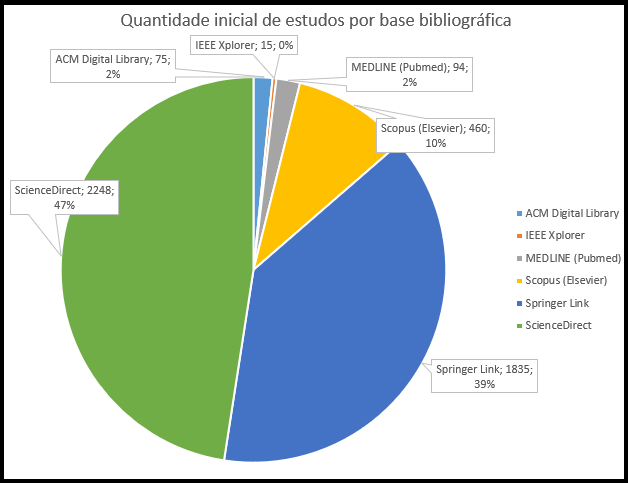
\includegraphics[scale=0.55]{Imagens/grafico - selecao inicial de estudos por base.png}
	\end{center}
	\legend{Fonte: Autor.}
\end{figure}

Além disso, o termo \textit{nutrition} estava associado a uma grande quantidade de estudos relacionados à técnicas de nutrição animal e medições de nutrientes vegetais, que não são relevantes para este trabalho. Estes resultados foram avaliados por seus resumos na etapa de inclusão e 2.625 estudos não foram incluídos para avaliações mais significativas. É possível conferir o comparativo de resultados por \textit{strings} de busca na \autoref{fig_graficoSelecaoInicialEstudosStrings}.

\begin{figure}[htb]
	\caption{\label{fig_graficoSelecaoInicialEstudosStrings}Gráfico de seleção inicial de estudos por \textit{strings} de busca.}
	\begin{center}
	    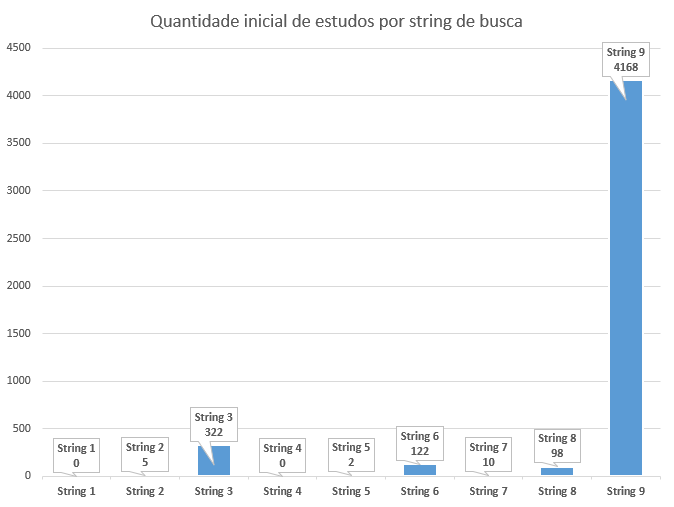
\includegraphics[scale=0.63]{Imagens/grafico - selecao inicial de estudos por string.png}
	\end{center}
	\legend{Fonte: Autor.}
\end{figure}

\begin{figure}[htb]
	\caption{\label{fig_graficoProcessoInclusaoExclusaoArtigos}Gráfico do processo de seleção dos estudos.}
	\begin{center}
	    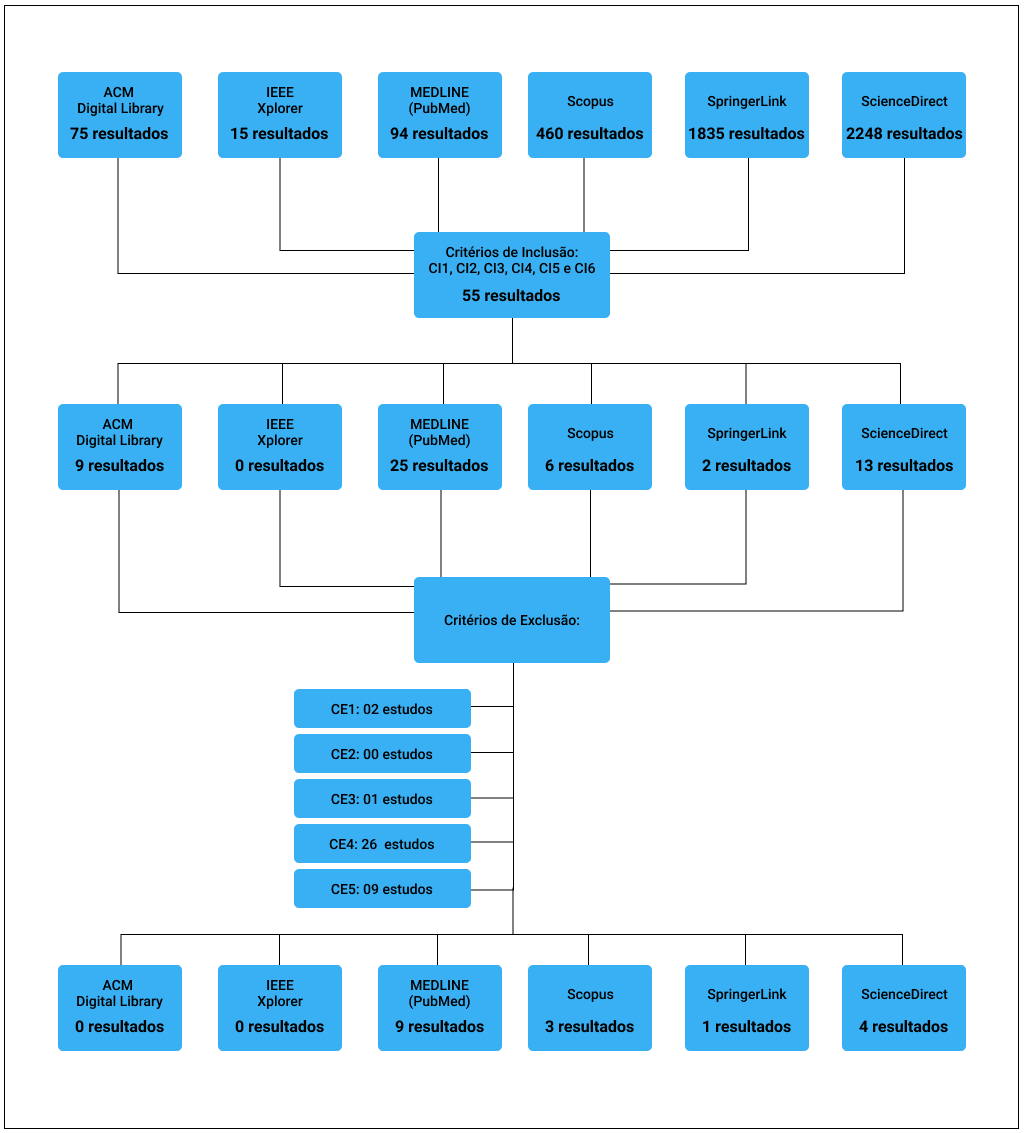
\includegraphics[scale=0.4]{Imagens/grafico - processo de selecao dos estudos.png}
	\end{center}
	\legend{Fonte: Autor.}
\end{figure}

\begin{figure}[htb]
	\caption{\label{fig_graficoResultadoProcessoExclusao}Resultado do processo de exclusão dos artigos.}
	\begin{center}
	    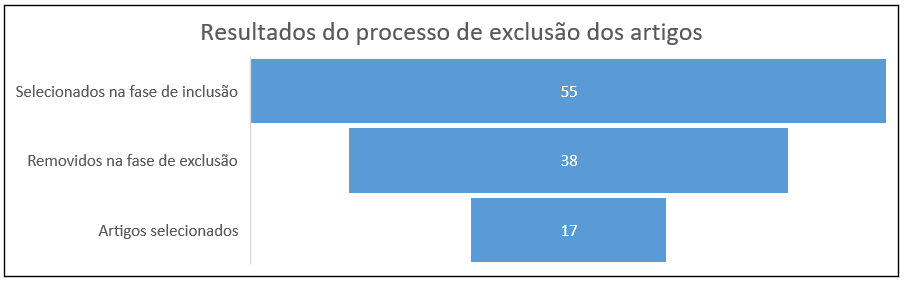
\includegraphics[scale=0.6]{Imagens/grafico - resultado da fase de exclusao dos artigos.png}
	\end{center}
	\legend{Fonte: Autor.}
\end{figure}

Após a execução da busca inicial de estudos, na etapa seguinte analisando os títulos e resumos, 55 resultados satisfizeram ao menos um dos critérios de inclusão e foram selecionados como estudos primários, como mostra a \autoref{fig_graficoProcessoInclusaoExclusaoArtigos}. 
\newline
\newline
\newline

Na etapa de exclusão, mostrada na \autoref{fig_graficoProcessoInclusaoExclusaoArtigos}, os artigos que foram coincidentes com ao menos um dos critérios de exclusão foram removidos da revisão. Do total de estudos primários, 26 resultados foram retirados por estarem duplicados, 11 estudos foram removidos por não tratarem do tema abordado neste trabalho e 17 artigos foram selecionados. A \autoref{fig_graficoResultadoProcessoExclusao} apresenta a quantidade total de artigos excluídos e aceitos para análise e extração dos dados. Os artigos selecionados são apresentados no \autoref{quadro_artigosSelecionados}.

\begin{quadro}[htb]
\caption{\label{quadro_artigosSelecionados}Artigos selecionados.}
\begin{tabular}{|p{1,5cm}|p{7cm}|p{5cm}|}
	\hline
	\textbf{Sigla} & \textbf{Título} & \textbf{Autores} \\ \hline
	A1  & \textit{A dietary assessment app for hospitalized patients at nutritional risk:Development and evaluation of the myfood app} & \cite{paulsen2018_1} \\ \hline
	A2  & \textit{A Parenteral Protein Decision Support System Improves Protein Delivery in Preterm Infants: A Randomized Clinical Trial} & \cite{alrifai2017} \\ \hline
	A3  & \textit{A validation of an intelligent decision-making support system for the nutrition diagnosis of bariatric surgery patients} & \cite{cruz2017} \\ \hline
	A4  & \textit{Advancing competitive position in healthcare: a hybrid metaheuristic nutrition decision support system} & \cite{ileri2019} \\ \hline
	A5  & \textit{Assessing the feasibility of a mobile health-supported clinical decision support system for nutritional triage in oncology outpatients using Arden Syntax} & \cite{bruin2018} \\ \hline
	A6  & \textit{Barriers and Facilitators for Implementing a Decision Support System to Prevent and Treat Disease-Related Malnutrition in a Hospital Setting: Qualitative Study} & \cite{paulsen2018_2} \\ \hline
	A7  & \textit{Clinical Data Warehousing for Evidence Based Decision Making} & \cite{narra2015} \\ \hline
\end{tabular}
\end{quadro} 

\begin{quadro}[htb]
%\caption{(Continuação)}
%\label{}
\begin{tabular}{|p{1,5cm}|p{7cm}|p{5cm}|}
    \hline
	A8  & \textit{Concurrence of big data analytics and healthcare: A systematic review}& \cite{metha2018} \\ \hline
	A9  & \textit{Developing a standardized healthcare cost data warehouse} & \cite{visscher2017} \\ \hline
	A10  & \textit{E-assisted Nutrition Package for Hypertension Patients}& \cite{boonapai2016} \\ \hline
	A11 & \textit{Effects of using the MyFood decision support system on hospitalized patients' nutritional status and treatment: A randomized controlled trial} & \cite{paulsen2020} \\ \hline
	A12  & \textit{Impact of a computer-assisted decision support system (CDSS) on nutrition management in critically ill hematology patients: the NUTCHOCO study (nutritional care in hematology oncologic patients and critical outcome)} & \cite{ettori2019} \\ \hline
	A13  & \textit{Nutritional Alert in hospitalized patients} & \cite{brieux2014} \\ \hline
	A14  & \textit{Physicians' perceptions about managing enteral nutrition and the implementation of tools to assist in nutritional decision-making in a paediatric intensive care unit}& \cite{moullet2020} \\ \hline
	A15  & \textit{Requirements Analysis for a Clinical Decision Support System Aiming at Improving the Artificial Nutrition of Critically Ill Patients}& \cite{schuttler2017} \\ \hline
	A16  & \textit{Using a Web-Based Nutrition Algorithm in Hemodialysis Patients} & \cite{steiber2015} \\ \hline
	A17  & \textit{Using clinical decision support through the electronic medical record to increase prescribing of high-dose parenteral thiamine in hospitalized patients with alcohol use disorder} & \cite{wai2019} \\ \hline
\end{tabular}
\legend{Fonte: Autor.}
%\fonte{Autor.}
\end{quadro} 

Os artigos analisados pertencem a uma faixa de publicação entre os anos de 2014 e 2020. Na \autoref{fig_graficoQuantidadeArtigoAno} é apresentado um gráfico com a quantidade de artigos analisados por ano de publicação.
\newline
\newline
\newline
\newline
\newline
\newline
\newline

\begin{figure}[htb]
	\caption{\label{fig_graficoQuantidadeArtigoAno}Quantidade de artigos por ano de publicação.}
	\begin{center}
	    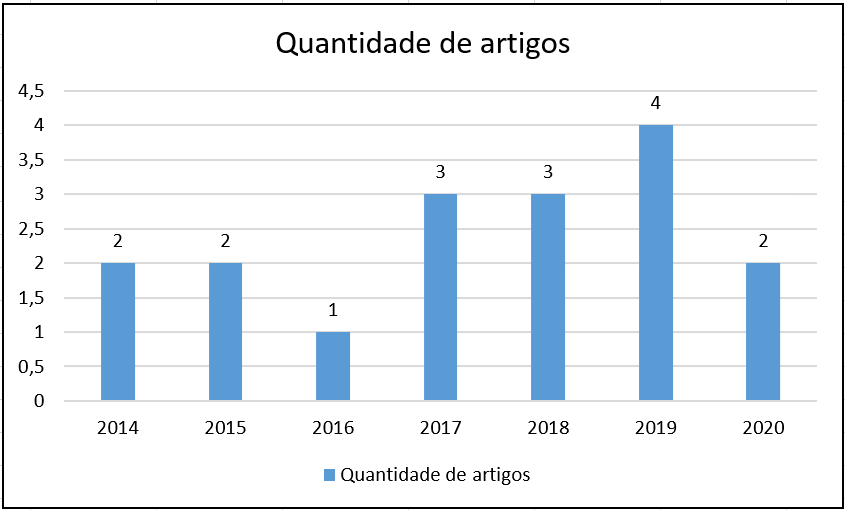
\includegraphics[scale=0.6]{Imagens/grafico - quantidade de artigos por ano de publicacao.png}
	\end{center}
	\legend{Fonte: Autor.}
\end{figure}

A maior quantidade de artigos analisados foram publicados no ano de 2019, com um total de 4 (quatro) artigos. Os anos de 2017 e 2018 apresentaram a segunda maior quantidade de publicações, sendo 3 (três) artigos em cada ano. Seguidos dos anos de 2014, 2015 e 2020 com 2 (dois) artigos em cada ano. E 1 (um) artigo no ano de 2016.

\section{Análise dos resultados}
Na fase de análise, uma vez selecionados os estudos, foi realizada a extração de informações relevantes. Esta seção apresenta as respostas obtidas para as questões de pesquisa. O \autoref{quadro_funcionalidadesArtigos} mostra as principais abordagens encontradas e as formas utilizadas para gerenciamento dos dados.

\textit{µ1: Como as pesquisas tratam o gerenciamento e a análise dos dados clínicos sobre o acompanhamento nutricional dos pacientes nos hospitais?}

\begin{quadro}[htb]
\caption{\label{quadro_funcionalidadesArtigos}Identificação das abordagens de gerenciamento e análise.}
\label{}
\begin{tabular}{|p{11cm}|p{4cm}|}
	\hline
	\textbf{Abordagem utilizada}   &   \textbf{Artigos}\\ \hline
	Apresenta relatório de dados probabilísticos gerados com redes Bayesianas.   &   A3, A4.\\ \hline
	Utiliza algoritmo genético e algoritmo de cozimento simulado para gerar recomendações nos relatórios.  &   A4.\\ \hline
	Utiliza dispositivo móvel para apresentar dados das avaliações nutricionais. & A1, A5, A6, A11.\\ \hline
	Apresenta \textit{Dashboard} com dados das avaliações nutricionais. & A1, A5, A10, A15, A17.\\ \hline
\end{tabular}
\end{quadro}

\begin{quadro}[htb]
\begin{tabular}{|p{11cm}|p{4cm}|}
    \hline
    Utiliza aplicação web para apresentar dados de avaliação nutricional. & A1, A5, A6, A10, A11.\\ \hline
	Possui estrutura de armazenamento de dados em\textit{ Data Warehouse}. & A7, A11.\\ \hline
	Utiliza \textit{plugin} para apresentar dados de avaliação nutricional.  & A2.\\ \hline
\end{tabular}
\legend{Fonte: Autor.}
%\fonte{Autor.}
\end{quadro}

Buscando responder a segunda questão de pesquisa, o \autoref{quadro_indicadoresArtigos} apresenta os formatos de aquisição de KPI utilizados pelos estudos.

\textit{µ2: Como os hospitais extraem indicadores-chave de desempenho (ICD) para análise de dados de acompanhamento nutricional?}

\begin{quadro}[htb]
\caption{\label{quadro_indicadoresArtigos}Formatos de aquisição de Indicadores-chave de desempenho.}
\label{}
\begin{tabular}{|p{11cm}|p{4cm}|}
	\hline
	\textbf{Abordagem utilizada}   &   \textbf{Artigos}\\ \hline
	Utiliza formulário integrado ao módulo de apoio a decisão. &  A2\\ \hline
	Utiliza dispositivo móvel para realizar preenchimento dos dados de avaliação nutricional. & A6, A11\\ \hline
	Utiliza aplicação web para realizar preenchimento de formulário dos dados de avaliação nutricional. & A1, A5 A10, A11\\ \hline
	Utiliza planilha eletrônica para carga de dados & A4, A7.\\ \hline
	Utiliza consulta a base de dados do sistema de administração hospitalar. & A10, A11, A12 A16, A17.\\ \hline
\end{tabular}
\legend{Fonte: Autor.}
%\fonte{Autor.}
\end{quadro}

O \autoref{quadro_ImpactosPositivos} apresenta a síntese sobre os impactos que cada artigo causou em seus respectivos ambientes de estudo. 
\newline

\textit{µ3: De que forma esses dados são utilizados e impactam na tomada de decisão dos setores assistenciais e de gestão dos estabelecimentos hospitalares?}

\begin{quadro}[htb]
\caption{\label{quadro_ImpactosPositivos}Síntese sobre os impactos positivos e negativos extraídos nos estudos.}
\label{}
\begin{tabular}{|p{1,5cm}|p{13,5cm}|}
	\hline
	\textbf{Artigo}   &   \textbf{Impactos}\\ \hline
	A1  &  Segundo \citeonline{paulsen2018_1} os dados fornecidos podem contribuir para prevenir o desenvolvimento de desnutrição relacionada à doença entre pacientes em risco.\\ \hline
	A2  &  Para \citeonline{alrifai2017} os principais pontos positivos foram o aumento significativo na dosagem apropriada, a melhora de uremia e o ganho de peso durante fase de nutrição enteral.\\ \hline
	A3  &  \citeonline{cruz2017} apresentam grande vantagem na sugestão de risco de desenvolvimento de doença com base nos relatórios.\\ \hline
	A4  & \citeonline{ileri2019} analisam os pedidos do menu de dieta e sugerem vários menus para fornecer eficácia de custo e possíveis taxas de erro mais baixas e ao mesmo tempo.\\ \hline
\end{tabular}
\end{quadro}
\newpage
\begin{quadro}[htb]
\begin{tabular}{|p{1,5cm}|p{13,5cm}|}
    \hline
	A5  &  \citeonline{bruin2018} apresentam um monitoramento que pode servir como o elo que faltava na identificação precoce de mudança no estado nutricional de um paciente.\\ \hline
    A6  & \citeonline{paulsen2018_2} apresentam um aplicativo móvel para acompanhamento nutricional de pacientes hospitalizados, que foi percebido pelos usuários como mais preciso, confiável, divertido e motivacional do que a prática tradicional. Contudo, aspectos culturais, de idioma, idade, higiene e falta de integração com sistema de prontuários foram percebidos como barreiras potenciais. \\ \hline
    A7 & \citeonline{narra2015} consideraram a vantagem de integrar diferentes fontes de dados para possibilitar análise dimensional. Além disso, a natureza não volátil dos \textit{Data Warehouses} permitem o estudo de vários fatores e problemas de saúde que só podem ser identificados com dados de um longo período de tempo além da possibilidade de aplicar técnicas de mineração de dados.\\ \hline
    A8 & \citeonline{metha2018} apresentam como o sistema de apoio à decisão ajuda na detecção precoce de doenças, dicção da trajetória da doença e identificação de desvio de estado saudável. O tratamento pode ser direcionado ajudando as organizações de saúde em custo-benefício e redução do desperdício de recursos.\\ \hline
    A9 & Em \citeonline{visscher2017}, um \textit{Data Warehouse} padronizado e baseado em provedor de dados de custos de saúde pode ser mantido facilmente. Sendo útil para fornecer estimativas de custo total razoáveis e compreensíveis, entendendo melhor o faturamento e possibilitando estratégias que melhorem o custo-benefício por paciente na rede hospitalar.\\ \hline
    A10 & \citeonline{boonapai2016} implementam com sucesso um modelo de consciência nutricional e orientação para o usuário, especialmente com hipertensão, diabetes e obesidade, porque podem controlar e monitorar sua condição e seus planos de dieta.\\ \hline
    A11 & \citeonline{paulsen2020} obtiveram um efeito significativo na proporção de pacientes com tratamento nutricional documentado no prontuário eletrônico do paciente.\\ \\ \hline
    A12 & \citeonline{ettori2019} mostraram melhorar relativamente a taxa de dias no cumprimento das metas calóricas e proteicas em mais de 50\%.\\ \hline
    A13 & O sistema de alerta apresentado por \citeonline{brieux2014} teve alta sensibilidade e especificidade e esse fato ajudou os médicos a diagnosticarem a desnutrição nos pacientes.\\ \hline
    A14 & Médicos relataram práticas mais consistentes e sistemáticas, segundo \citeonline{moullet2020}, como por exemplo, a determinação de metas de energia na admissão na Unidade de Terapia Intensiva Pediátrica e maior atenção à nutrição.\\ \hline
    A15 &  \citeonline{schuttler2017} propuseram três camadas de visualização, o que permitiu ao usuário obter as informações necessárias e, simultaneamente, evitar a sobrecarga de informações.\\ \hline
    A16 & \citeonline{steiber2015} apresentaram a capacidade de rastrear mudanças nas medidas de avaliação ao longo do tempo. \\ \hline
\end{tabular}
\end{quadro}
\newpage
\begin{quadro}[htb]
\begin{tabular}{|p{1,5cm}|p{13,5cm}|}
    \hline
    A17 & O trabalho realizado por \citeonline{wai2019} resultou em um aumento significativo na prescrição de tiamina parenteral em alta dose e uma tendência à significância estatística para diminuir o tempo de internação. \\ \hline
\end{tabular}
\legend{Fonte: Autor.}
%\fonte{Autor.}
\end{quadro}
Também buscando responder a terceira questão de pesquisa, foi identificada a densidade de KPI utilizadas nos artigos, conforme a \autoref{fig_graficoDensidadeKPI}.

\begin{figure}[htb]
	\caption{\label{fig_graficoDensidadeKPI}Densidade de KPI identificadas na RS.}
	\begin{center}
	    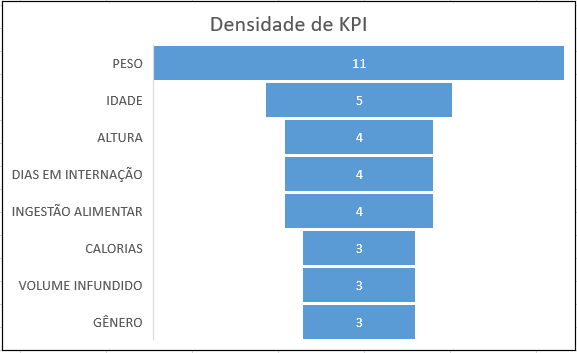
\includegraphics[scale=0.8]{Imagens/grafico - densidade de kpi.png}
	\end{center}
	\legend{Fonte: Autor.}
\end{figure}


\section{Considerações finais do capítulo}
Este capítulo descreveu a execução de cada etapa do processo da revisão sistemática. Esta revisão teve como objetivo conhecer as pesquisas que trataram do apoio a tomada de decisão na área da nutrição hospitalar. Foi apresentado o processo de planejamento e realização da execução da revisão, por fim, realizada a extração dos dados, obtendo as principais abordagens de gerenciamento e análise dos dados, formas de extração e principais KPI utilizados em projetos de sistemas de apoio à decisão. No próximo capítulo será descrito o desenvolvimento da solução de \textit{Business Intelligence} da Unidade de Nutrição do HU.